\chapter{Lecture 27: Multi-variate continuous distributions and conditional probabilities}

\section{Multi-variate continuous distributions} \label{jointly continuous} \label{joint cumulative distribution function} \label{joint probability density function}  \label{f(x,y) symbol}
\label{F(x,y) symbol}
Two (or more) random variables are referred to as \textbf{jointly continuous} when they have a \textbf{joint cumulative distribution function} ($F(x,y)$, defined in the following box) which is continuous in both variables:

  	\bigskip
	
	\hfil\fbox{
	\begin{minipage}{0.4\columnwidth}{
	
	\vskip 0.04cm
	\begin{center}
	$\displaystyle{F(x,y) = \int_{-\infty}^x \int_{-\infty}^y f(s,t) \; dtds}$
	\end{center}
	}
	\end{minipage}}
	\bigskip
	\bigskip

\noindent The function, $f(x,y)$, is called the \textbf{joint probability density function}. In the above integral, $s$ is a dummy variable taking the place of $x$, and $t$ is a dummy variable taking the place of $y$. \\

\noindent The probabilty that $X$ falls in the interval $[a,b]$ \textit{and} $Y$ falls in the interval [$c,d$] is given by

  	\bigskip
	
	\hfil\fbox{
	\begin{minipage}{0.58\columnwidth}{
	
	\vskip 0.04cm
	\begin{center}
	$\displaystyle{P(a \leq X \leq b, c \leq Y \leq d) = \int_a^b\int_c^d f(x,y) \; dy dx}$
	\end{center}
	}
	\end{minipage}}
	\bigskip
	\bigskip

\noindent In section \ref{double integral} we learned that the graph of $f(x,y)$ can be interpreted as a surface. We also learned to interpret the above double integral as the \textit{volume} between the surface, $f(x,y)$, and a section of the $x,y$-plane. For joint probability density functions of more than two variables, we can no longer visualise the graph in three dimensions, so trying to think of such probabilities graphically is not generally productive. \\

\noindent To satisfy the probability measure axioms, a joint pdf and joint cdf must fulfill the following requirements. Pay attention to the use of `\textit{and}' as well as the use of `\textit{or.}'
\begin{itemize}
\item As $x \rightarrow -\infty$ \textit{or} $y \rightarrow -\infty$, $F(x,y) \rightarrow 0$.
\item As $x \rightarrow \infty$ \textit{and} $y \rightarrow \infty$, $F(x,y) \rightarrow 1$.
\item $f(x,y) \geq 0$ for all $x,y$.
\end{itemize}
It makes sense that we have used `\textit{or}' where we did, since, for example, the probability that $X$ takes on any value in its range \textit{and} $Y$ takes on a value outside of its range, must still be equal to zero (since $Y$ cannot take on a value outside of its range). It also makes sense that we used `\textit{and}' where we did, since integrating over all possible values of \textit{both} random variables is equivalent to asking for $P(\Omega)$, which we know is equal to $1$. \\

\noindent Note that the first requirement (that $F(x,y) \rightarrow 0$ when $x \rightarrow -\infty$ or $y \rightarrow -\infty$), follows directly from the definition of $F(x,y)$ since it is always true that the integral from $-\infty$ to $-\infty$ must be equal to zero, i.e.,
\[
\int_{-\infty}^{-\infty} \int_{-\infty}^y f(s,t) \; dtds = 0, \qquad \text{and} \qquad \int_{-\infty}^x \int_{-\infty}^{-\infty} f(s,t) \; dt ds = 0.
\]

\noindent Hence, in the following example, we only check the second two requirements.

\subsection{Example} \label{ex27.1}
Let $k$ be some real number. Suppose that the jointly continuous random variables, $X$ and $Y$, have a joint probability density function given by
\[
f(x,y) = \left\{ \begin{array}{ll}
kxy & \; \text{if} \;\; x \in [0,1] \; \textit{and} \; y \in [0,1] \smallskip \\
0 & \; \text{otherwise}
\end{array} \right.
\]
\begin{enumerate}
\item Find the value of $k$ that makes this a joint pdf (i.e., the value of $k$ for which this function satisfies the probability measure axioms).
\item Find $F(x,y)$.
\item Calculate $P(X \leq 0.75, Y \geq 0.5)$.
\end{enumerate}
\bigskip

\solution[to (1)]
First of all, when $x \in [0,1]$ and $y \in [0,1]$ we get $f(x,y) \geq 0$ whenever $k \geq 0$, so we require that $k$ is non-negative. \\

\noindent The other requirement is that $\int_{-\infty}^\infty \int_{-\infty}^\infty f(x,y) \; dy dx = 1$, i.e., 
\[
\int_{0}^1 \int_{0}^1 kxy \; dy dx = 1. \tag{since $f(x,y) = 0$ whenever $x \notin [0,1]$ or $y \notin [0,1]$}
\]
Evaluating the `inner' integral gives
\[
\int_{0}^1 \squac{kx\frac{y^2}{2}}^1_{0} \; dx = \int_{0}^1 kx\frac{1}{2} \; dx = 1.
\]
Now, evaluating the `outer' integral gives
\[
\int_{0}^1 kx\frac{1}{2} \; dx = \squac{k\frac{x^2}{4}}_0^1 = \frac{k}{4} = 1.
\]
So we must have $\frac{k}{4} = 1$. Hence $k = 4$. \\

\solution[to (2)]
Using the definition of a joint cdf, $F(x,y)$, we have
\begin{align*}
F(x,y) & = \int_{-\infty}^x \int_{-\infty}^y f(s,t) \; dtds \tag{by definition}  \\
	& = \int_{0}^x\int_0^y kst \; dtds \tag{since $f(x,y) = 0$ whenever $x \notin [0,1]$ or $y \notin [0,1]$} \\
	& = \int_0^x \squac{ks\frac{t^2}{2}}_0^y \; ds \tag{integrating with respect to $t$} \\
	& = \int_0^x ks\frac{y^2}{2} \; ds \\
	& = k\frac{x^2y^2}{4} \tag{integrating with respect to $s$} \\
	& = x^2y^2. \tag{since we found $k = 4$ in part (1)}
\end{align*}
So we have
\[
F(x,y) = x^2y^2, \;\;\; \text{for $x \in [0,1]$ and $y \in [0,1].$}
\]
Technically, we have to consider all possible cases for $x$ and $y$, to fully define the joint cdf. Since $f(x,y) = 0$ when either $x$ or $y$ is not in $[0,1]$, the value of $y$ in the cdf reaches its maximum at $y = 1$, and similarly, the value of $x$ reaches its maximum when $x = 1$. So we get
\[
F(x,y) = \left\{ \begin{array}{ll}
1	& \;\text{if} \;\; x \geq 1 \; \text{and} \; y \geq 1  \smallskip \\
x^2	& \;\text{if} \;\; x \in [0,1] \; \text{and} \; y \geq 1  \smallskip \\
y^2	& \;\text{if} \;\;  x \geq 1 \; \text{and} \; y \in [0,1] \smallskip \\
x^2y^2 & \;\text{if} \;\;  x \in [0,1] \; \text{and} \; y \in [0,1] \smallskip \\
0	& \; \text{otherwise (i.e., if $x \leq 0$ or $y \leq 0$ or both)}
\end{array} \right.
\]
To convince yourself that these cases are correct, consider the fact that, for example 
\begin{align*}
\int_0^\infty \int_0^y f(x,t) \; dtdx & = \int_0^1 \int_0^y f(x,t) \; dtdx + \int_1^\infty \int_0^y f(x,t) \; dtdx \\
& = \int_0^1 \int_0^y f(x,t) \; dtdx + 0. \tag{since $f(x,y) = 0$ when $x \geq 1$} \\
& = \int_0^1 \int_0^y 4xt \; dtdx \tag{since $k = 4$ by part (1)} \\
& = \int_0^1 4x\frac{y^2}{2} \; dx \\
& = y^2.
\end{align*}
So $F(x,y) = y^2$ when $x \geq 1$ and $y \in [0,1]$. \\

\solution[to (3)]
We have $0.75 = 3/4$ and $0.5 = 1/2$. Now,
\begin{align*}
P(X \leq 0.75, Y \geq 0.5) & = \int_{-\infty}^{\frac{3}{4}} \int_{\frac{1}{2}}^{\infty} f(x,y) \; dy dx \\
	& = \int_{0}^{\frac{3}{4}} \int_{\frac{1}{2}}^{1} 4xy \; dydx \tag{since $f(x,y) = 0$ elsewhere} \\
	& = \int_{0}^{\frac{3}{4}} \squac{2xy^2}_{\frac{1}{2}}^1 \; dx \\
	& = \int_{0}^{\frac{3}{4}} 2x - \frac{x}{2} \; dx \\
	& = \squac{x^2 - \frac{x^2}{4}}_0^{\frac{3}{4}} \\
	& = \frac{27}{64}. \tag{notice that $x^2 - \frac{x^2}{4} = x^2\brac{1-\frac{1}{4}} = x^2\frac{3}{4}$}
\end{align*}

\noindent For your interest, the graph of $f(x,y)$ is pictured below (it is a `sail'-like surface):
\begin{center}
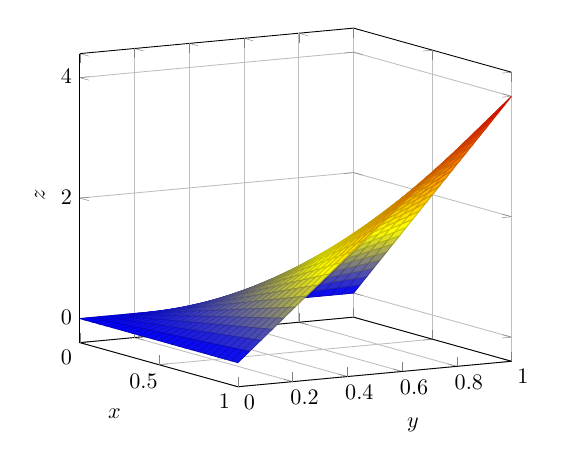
\begin{tikzpicture}[scale=0.8]
\begin{axis}[grid=both,
xlabel={$x$},
ylabel={$y$},
zlabel={$z$},
view={60}{10}
]
\addplot3[surf,domain=0:1,shader=faceted] {4*\x*\y};
\end{axis}
\end{tikzpicture}
\end{center}

\noindent Notice that the section of the $x,y$-plane pictured is the section where $x \in [0,1]$ and $y \in [0,1]$ (this is the only section where $f(x,y)$ can be non-zero).

\subsection{Marginal pdfs for jointly continuous distributions} \label{marginal probability density function 2} \label{f_X(x) symbol}
Recall that for a discrete bi-variate joint distribution of two random variables, $X$ and $Y$, the marginal pmfs were defined (in section \ref{marginal probabilities}) as 
\[
p_X(x_i) = \sum_j p(x_i,y_j) \qquad \text{and} \qquad p_Y(y_j) = \sum_i p(x_i,y_j)
\]
The marginal pmf for one variable is found by summing the joint pmf over all possible values of the \textit{other} variable. Similarly, for a bi-variate jointly continuous distribution, the \textbf{marginal probability density function} of one variable is found by integrating over all possible values of the \textit{other} variable:
  
  	\bigskip
	
	\hfil\fbox{
	\begin{minipage}{0.75\columnwidth}{
	
	\vskip 0.04cm
	\begin{center}
	$\displaystyle{f_X(x) = \int_{-\infty}^\infty f(x,y) \; dy \qquad \text{and} \qquad f_Y(y) = \int_{-\infty}^\infty f(x,y) \; dx}$
	\end{center}
	}
	\end{minipage}}
	\bigskip
	\bigskip
	
\subsection{Example} \label{ex27.3}
For the joint pdf from the previous example, example \ref{ex27.1}, find the marginal pdfs, $f_Y(y)$ and $f_X(x)$. \\

\solution
Using the definition in the box above for marginal pdfs we have
\begin{align*}
f_X(x) & = \int_{-\infty}^\infty f(x,y) \; dy \\
	& = \int_0^1 4xy \; dy \tag{since $f(x,y) = 0$ when $y \notin [0,1]$} \\
	& = \squac{2xy^2}_0^1 \\
	& = 2x.
\end{align*}
A similar process gives $f_Y(y) = 2y$.

\section{Conditional probabilities (discrete)} \label{discrete conditional probability}
In section \ref{sec508} we gave the definition of conditional probability (the probability of event $A$ given that event $B$ has occurred): 
\[
P(A|B) = \frac{P(A \cap B)}{P(B)}.
\]
Thus far, we have not shown how this definition can be applied to (discrete or continuous) random variables. It is easy to adapt this definition to discrete random variables, keeping in mind how we use random variables to specify events; we can replace the arbitrary event $A$ with $\set{X = x_i}$, and replace $B$ with $\set{Y = y_i}$. Then the above gives us
\[
P(\set{X = x_i} \mid \set{Y = y_i}) = \frac{P(\set{X = x_i} \cap \set{Y = y_i})}{P(\set{Y = y_i})}
\]
Usually we write this less formally as: 
  
  	\bigskip
	
	\hfil\fbox{
	\begin{minipage}{0.55\columnwidth}{
	
	\vskip 0.04cm
	\begin{center}
	$\displaystyle{P(X = x_i \mid Y = y_i) = \frac{P(X = x_i, Y = y_i)}{P(Y = y_i)}}$
	\end{center}
	}
	\end{minipage}}
	\bigskip
	\bigskip
	
\noindent We have waited until now to introduce conditional probabilities with random variables because we need to consider the joint probabilities $P(X = x_i, Y = y_i)$ of two different random variables, $X$ and $Y$, for the above to make sense. \\

\noindent It is often convenient to express the above in terms of probability mass functions. For this we will need to introduce the following new notation. We use: \label{p_{XY}(x,y),p_{X|Y}(x|y),p_X(x)}
\begin{itemize}
\item $\boldsymbol{p_{XY}(x,y)}$ for the joint probability mass function of $X$ and $Y$ (which gives $P(X = x,Y=y)$) previously we just used $p(x,y)$ to represent this (we just add the $XY$ subscript now, but it means the same thing as $p(x,y)$ did).
\item $\boldsymbol{p_{X|Y}(x|y)}$ for the probability mass function of $X$ conditional on $Y$ (which gives $P(\set{X = x}|\set{Y = y})$
\item $\boldsymbol{p_X(x)}$ for the marginal probability mass function of $X$ (and also $p_Y(y)$ for $Y$)
\end{itemize}

\noindent Using this notation, we can rewrite the expression in the box above as
  
  	\bigskip
	
	\hfil\fbox{
	\begin{minipage}{0.4\columnwidth}{
	
	\vskip 0.04cm
	\begin{center}
	$\displaystyle{p_{X|Y}(x|y) = \frac{p_{XY}(x,y)}{p_Y(y)}}$
	\end{center}
	}
	\end{minipage}}
	\bigskip
	\bigskip
	
\noindent Recall that $P(A|B)$ is undefined when $P(B) = 0$ (since the definition would otherwise require that we divide by zero). In the case of discrete random variables we use the convention that $p_{X|Y}(x|y) = 0$ when $p_Y(y) = 0$, rather than allowing the function to become undefined. \label{sec27.2}



\subsection{Example} \label{ex27.4}
In section \ref{p(x_i,y_j)=P(X=x_i,Y=y_j)}, we introduced an example in which a fair coin is tossed three times: Letting $X$ be the number of heads on the first toss, and letting $Y$ be the total number of heads (in the three tosses). \\

\noindent We then filled out the array below, which gives the joint probability mass function (and the marginal probabilities) for $X$ and $Y$.
\[
\begin{array}{cc|cccc|c} 
%top label
&& \multicolumn{3}{c}{\boldsymbol{y}} & \\
%second label
&& \multicolumn{1}{c}{0} &  \multicolumn{1}{c}{1} &  \multicolumn{1}{c}{2} &  3 & p_X(x_i) \\ \hline
%row 1
$$\boldsymbol{x}$$ \multirow{3}{*}{$$} &0& \frac{1}{8} & \frac{2}{8} & \frac{1}{8} & 0 &\boldsymbol{\frac{1}{2}}  \\ 
%row 2
&1&  0                 & \frac{1}{8} & \frac{2}{8} & \frac{1}{8} & \boldsymbol{\frac{1}{2}} \\ \hline
%row 3           
\multicolumn{1}{c}{p_Y(y_j)} &&\boldsymbol{\frac{1}{8}}&\boldsymbol{\frac{3}{8}}&\boldsymbol{\frac{3}{8}}&\boldsymbol{\frac{1}{8}}
\end{array}
\]
Using this array, find the probability that $X = 1$ given that $Y = 2$. Also, what is the probability that $Y = 2$ given that $X = 1$? \\

\solution
We need to find $p_{X|Y}(1,2)$ (the probability that $X = 1$ given that $Y = 2$). From the table we have $p_{XY}(1,2) = \frac{2}{8}$ (the probabiliy that $X = 1$ and $Y = 2$). Also from the table (in the lower margin) we have $p_Y(2) = \frac{3}{8}$ (the probability that $Y = 2$). Hence, using the definition of conditional probability
\[
p_{X|Y}(1,2) = \frac{2/8}{3/8} = \frac{2}{3}.
\]
The question also asks us for $p_{X|Y}(2,1)$. Using the table again we get
\[
p_{X|Y}(2,1) = \frac{p_{XY}(2,1)}{p_X(1)} = \frac{2/8}{1/2} = \frac{1}{2}.
\]

\subsection{$\boldsymbol{p_{X|Y}(x,y)}$ is a probability mass fuinction}
To check that $p_{X|Y}(x,y)$ satisfies the conditions to be a probability mass function, we need to check that
\begin{enumerate}
\item $\displaystyle{\sum_xp_{X|Y}(x|y) = 1}$ \;\; (i.e., probability measure axiom 1)
\item $\displaystyle{p_{X|Y}(x|y) \geq 0}$ \;\; (i.e., probability measure axiom 2)
\end{enumerate}
\smallskip
\noindent \textbf{Check (1):} \\
By the definition of conditional probability we have
\begin{align*}
\sum_xp_{X|Y}(x|y) & = \sum_x \frac{p_{XY}(x,y)}{p_Y(y)} \\
	& = \frac{1}{p_Y(y)} \sum_x p_{XY}(x,y) \tag{since we sum with respect to $x$, not $y$} \\
	& = \frac{1}{p_Y(y)} p_Y(y) \tag{by definition of the marginal pmf $p_Y(y)$} \\
	& = 1, \;\;\; \text{as required.}
\end{align*}
In the second last step we used the definition of the marginal pmf, which we gave (again) in section \ref{marginal probability density function 2}. The expression $p_{XY}(x,y)$ looks different to what appears in the definition in section \ref{marginal probability density function 2}, but $p_{XY}(x,y)$ is just different notation for the same thing as the previously used $p(x,y)$.  \\

\noindent \textbf{Check (2):} \\
Again, by the definition of conditional probability we have
\begin{align*}
p_{X|Y}(X|y) & = \frac{p_{XY}(x,y)}{p_Y(y)} \\
	& = \frac{P(X = x,Y = y)}{P(Y = y)}.
\end{align*}
Which is a ratio of two probabilities. Since probabilities are always positive, this ratio must also be positive. Hence $p_{X|Y}(x|y) \geq 0$, as required. Technically, we also need to consider the case where $p_Y(y) = 0$; for which $p_{X|Y}(x|y) = 0$ by definition (as stated on page \pageref{sec27.2}).

\subsection{Using law of total probability to find a marginal pmf}
Recall the law of total probability, which we derived in section \ref{law of total probability} (for some event $A$ and a family of exhaustive and mutually disjoint events $B_1,B_2,\ldots,B_n$):
\[
P(A) = \sum_{i = 1}^n P(A|B_i)P(B_i)
\]
Since the events specified by a random variable are (collectively) necessarily disjoint and exhaustive (see section \ref{sec8.10}), we can apply the law of total probability to discrete random variables (in a similar way to how we applied the definition of conditional probability). The family of events, $B_i$, are replaced by $\set{Y = y_j}$, and $A$ is replaced by $\set{X = x_i}$. So, in terms of pmfs we get
  
  	\bigskip
	
	\hfil\fbox{
	\begin{minipage}{0.4\columnwidth}{
	
	\vskip 0.04cm
	\begin{center}
	$\displaystyle{p_X(x) = \sum_{y}p_{X|Y}(x,y)p_Y(y)}$
	\end{center}
	}
	\end{minipage}}
	\bigskip
	\bigskip
	
\section{Conditional probabilities (continuous)} \label{f_{XY}(x,y),f_{X|Y}(x|y),f_X(x)}
Before we define conditional probability for continuous random variables, we need to introduce some new notation:
\begin{itemize}
\item $\boldsymbol{f_{XY}(x,y)}$ for the joint probability density function of $X$ and $Y$ (previously we just used $f(x,y)$ to represent this (we just add the $XY$ subscript now, but it means the same thing as $f(x,y)$ did).
\item $\boldsymbol{f_{X|Y}(x|y)}$ for the probability density function of $X$ conditional on $Y$.
\item $\boldsymbol{f_X(x)}$ for the marginal probability density function of $X$ (and also $f_Y(y)$ for $Y$)
\end{itemize}
It turns out that (for reasons somewhat outside the scope of this course) defining conditional probability on continuous random variables, $X$ and $Y$, is more difficult than might be expected. At first sight, the definition of the conditional pdf (below) \textit{looks} just like the definition of the conditional pmf for discrete random variables (only $p$ has been replaced by $f$):
  
  	\bigskip
	
	\hfil\fbox{
	\begin{minipage}{0.35\columnwidth}{
	
	\vskip 0.04cm
	\begin{center}
	$\displaystyle{f_{X|Y}(x|y) = \frac{f_{XY}(x,y)}{f_Y(y)}}$
	\end{center}
	}
	\end{minipage}}
	\bigskip
	\bigskip
	
\noindent In fact this appearance is deceptive: A more accurate way to write $f_{X|Y}(x|y)$ would be to write $f_{X|Y=y}(x|y)$, which is read ``the conditional probability density function of $X$ given that $Y$ takes \textit{some specific value}, $y$.'' The way that we recover probabilities from this conditional pdf is to use the following formula:
  
  	\bigskip
	
	\hfil\fbox{
	\begin{minipage}{0.55\columnwidth}{
	
	\vskip 0.04cm
	\begin{center}
	$\displaystyle{P(a \leq X \leq b \mid Y = y) = \int_a^b f_{X|Y}(x|y) \; dx}$
	\end{center}
	}
	\end{minipage}}
	\bigskip
	\bigskip

\noindent The fact that the definition of the conditional pdf requires that $Y$ take a specific value, and not some interval, has some grave implications for our current understanding of conditional probability in this course. \\

\noindent The problem is that (as we discussed in section \ref{subsec15.1}) there is always exactly zero probability that a continuous random variable will take some specific value. That is, $P(Y = y) = 0$, whenever $Y$ is continuous. Thus, it seems that $P(a \leq X \leq b \mid Y = y)$ is conditional on the impossible happening (we know that $P(A|B)$ makes no sense when $P(B) = 0$, and in this case we know that $P(Y = y) = 0$). \\

\noindent This problem is resolved in more advanced courses on probability, using limits. For now, we have to remain content that the definition of conditional probability for continuous random variables does not (apparently) agree with our general definition of $P(A|B)$ (of course, it does, we are just unable to give you a reason why here).

\subsection{Example} \label{ex27.5}
Using $f(x,y)$ from example \ref{ex27.1}, find $f_{X|Y}(x|y)$ and find $P(X \leq 0.75 \mid Y = 0.5)$. \\

\solution
For $x,y \in [0,1]$ we have $f_{XY}(x,y) = 4xy$ (using our previous result from the solution to (1) in example \ref{ex27.1}). Also, from the result in example \ref{ex27.3} we have $f_Y(y) = 2y$. Now, by the definition of the conditional pdf, we have
\begin{align*}
f_{X|Y}(x|y) = \frac{f_{XY}(x,y)}{f_Y(y)} = \frac{4xy}{2y} = 2x, \;\;\; \text{when $x,y \in [0,1]$}
\end{align*}
And $f_{X|Y}(x|y) = 0$ elsewhere. Now, the question also asks us to find $P\brac{X \leq 3/4 \mid Y = 1/2}$. Using the definition of conditional probability for continuous random variables we have
\begin{align*}
P(X \leq 3/4 \mid Y = 1/2) & = \int_{-\infty}^\frac{3}{4} f_{X|Y}\brac{x|1/2} \; dx \\
	& = \int_{0}^\frac{3}{4} 2x \; dx. \tag{letting $y = 1/2$ had no effect since $f_{X|Y}(x|y) = 2x$ did not depend on $y$} \\
	& = \squac{x^2}_0^\frac{3}{4} \\
	& = \frac{9}{16}.
\end{align*}

\subsection{Law of total probability for a marginal pdf}
Just as the law of total probability was a useful way to find the marginal pmf in a discrete joint distribution, it can also be used to give us the marginal pdf in a jointly continuous distribution. We can derive the law of total probability for jointly continuous random variables as follows. Solving for $f_{XY}(x,y)$ in the definition of a conditional pdf gives
\[
f_{XY}(x,y) = f_{X|Y}(x|y)f_Y(y) \tag{$\bigstar$}
\]
\noindent We already know the definition of $f_X(x)$ (the marginal pdf) from section \ref{marginal probability density function 2}:
\[
f_{X}(x) = \int_{-\infty}^\infty f_{XY}(x,y) \; dy
\]
Replacing $f_{XY}(x,y)$ in this equation with the expression on the right hand side of $\bigstar$ gives us the law of total probability for a marginal pdf:

  	\bigskip
	
	\hfil\fbox{
	\begin{minipage}{0.4\columnwidth}{
	
	\vskip 0.04cm
	\begin{center}
	$\displaystyle{f_X(x) =  \int_{-\infty}^\infty f_{X|Y}(x|y)f_Y(y) \; dy}$
	\end{center}
	}
	\end{minipage}}
	\bigskip
	\bigskip
 
\section{Conditional expected values} \label{conditional expected value} \label{E(X|Y = y)}
In section \ref{expected value} we introduced the expected value, $E(X)$, of a random variable, $X$. \textbf{Conditional expected values,} $\boldsymbol{E(X|Y=y)}$, are calculated by replacing the pmf or pdf by a conditional pmf or pdf; i.e., for discrete random variables we define

  	\bigskip
	
	\hfil\fbox{
	\begin{minipage}{0.4\columnwidth}{
	
	\vskip 0.04cm
	\begin{center}
	$\displaystyle{E(X|Y=y) = \sum_x xp_{X|Y}(x|y)}$
	\end{center}
	}
	\end{minipage}}
	\bigskip
	\bigskip
 
\noindent And for continuous random variables we define

  	\bigskip
	
	\hfil\fbox{
	\begin{minipage}{0.4\columnwidth}{
	
	\vskip 0.04cm
	\begin{center}
	$\displaystyle{E(X|Y=y) = \int_{-\infty}^\infty xf_{X|Y}(x|y) \; dx}$
	\end{center}
	}
	\end{minipage}}
	\bigskip
	\bigskip
	
\subsection{Example (discrete)}
Using the probability mass function from example \ref{ex27.4}, we found that $p_{X|Y}(1|2) = 2/3$ and we can find $p_{X|Y}(0,2) = 1/3$. Use these two results to find $E(X|Y = 2)$. \\

\solution
Using the definition of conditional expected value we have
\begin{align*}
E(X|Y = 2) & = \sum_x xp_{X|Y}(x|2) \\
	& = 0\times p_{X|Y}(0|2) + 1\times p_{X|Y}(1|2) \tag{since $x \in \set{0,1}$} \\
	& = \frac{2}{3}.
\end{align*}
 
\subsection{Example (continuous)}
Using $f(x,y)$ from example \ref{ex27.1}, find $E(X | Y = y)$, for any arbitrary $y$, using the fact, from the result in example \ref{ex27.5}, that $f_{X|Y}(x|y) = 2x$, when $x \in [0,1]$ and $f_{X|Y}(x|y) = 0$ elsewhere.  \\
 
\solution
Using the definition of conditional expected value we have
\begin{align*}
E(X | Y = y) & = \int_{-\infty}^\infty xf_{X|Y}(x|y) \; dx \\
	& =  \int_{0}^1  2x^2 \; dx \tag{since $f_{X|Y}(x|y) = 2x$ when $x \in [0,1]$} \\
	& = \squac{\frac{2}{3}x^3}_0^1 \\
	& = \frac{2}{3}.
\end{align*}
It is just a coincidence that this is the same number as the previous (discrete) example.